\documentclass{beamer}
\usepackage{ dsfont }
\usepackage[utf8]{inputenc}
\usepackage[english]{babel}
\setbeamersize{text margin left=10pt, text margin right=10pt} %new code
\usepackage{graphicx}
\usepackage{float}
\usepackage{subcaption}
\usefonttheme{professionalfonts} % using non standard fonts for beamer
\setbeamerfont{frametitle}{series=\bfseries}
\usepackage{animate}
\usepackage{movie15}
\usepackage{breqn, bm}
\usepackage{amsmath}
\usepackage[skins]{tcolorbox}
\usepackage{subcaption}

\definecolor{notgreen}{RGB}{255,127,0}
\definecolor{green}{RGB}{49,150,3}
\setbeamerfont{headline}{size=\small}


%----------------------------------------------------------------------------------------
%	 Package
%----------------------------------------------------------------------------------------
\usepackage{color}
\usepackage{url}
\beamertemplatenavigationsymbolsempty
\definecolor{cadmiumred}{rgb}{0.8, 0.8, 0.8}

%----------------------------------------------------------------------------------------
%	 Presentation settings
%----------------------------------------------------------------------------------------

\usetheme{default}
\usecolortheme{default}

\setbeamertemplate{itemize items}[triangle] 
\setbeamertemplate{enumerate items}[default]
 
\title[Variational Drop Out]{
	MIPT Data Visualization Course\\ 
	\vspace{1cm}
	\textbf{\textcolor{black}{Data Visualization in Modern Machine Learning}}}

\author{Ashuha Arseniy$^{1, 2}$}
\institute[Bayesgroup, MIPT]{
	Bayesian Research Group$^1$, MIPT$^2$\\
	
	\medskip
	
\includegraphics[scale=0.5]{./img/logo} 
\includegraphics[scale=0.12]{./img/mipt}
	
	\href{ars-ashuha.ru/slides}{ars-ashuha.ru/slides}}

\date{\today}

\newcommand{\Expect}{\mathsf{E}}
\newcommand{\MExpect}{\mathsf{M}}
\newcommand{\cov}{\mathsf{cov}}
\setbeamertemplate{section in toc}[circle]

\addtobeamertemplate{navigation symbols}{}{%
	\usebeamerfont{footline}%
	\usebeamercolor[fg]{footline}%
	\hspace{1em}%
	\insertframenumber/\inserttotalframenumber
}


\begin{document}
\begin{frame}
	\titlepage 
\end{frame}

\begin{frame}{Motivation}
	  Motivation 
	\begin{itemize}
		 \item It's a little bit sad, but we can plot only 2D data, isn't it?
		 \item A goal of data visualization is to understand inner data structure.
		  \item Or represent data in a much more interpretable form.
	\end{itemize}
	\vspace{1cm}
	 There are two way to get this goal:
	\begin{itemize}
		  \item Low Rank Way (SVD, Auto-encoders, LDA, etc.)
		  \item Generative Models Way (GAN, Image Capturing, etc.)
	\end{itemize}
\end{frame}

\begin{frame}{Low Rank idea}
	\begin{itemize}
		  \item We have matrix $X_{items \times features}$
		  \item Let's try to represent each item's vector as smaller ones.
		  \item What should we do? 
	\end{itemize}
	
	 Principal component analysis is a matrix decomposition
	
	\begin{center}
		 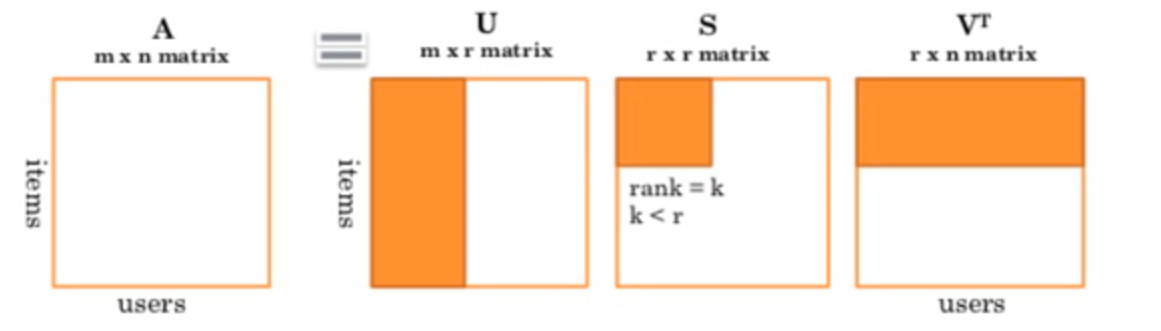
\includegraphics[scale=0.2]{img/svd}
	\end{center}
	
	 Intuition save maximum data variance,  minimize $L_2$ norm
	 
	 \begin{center}
	 	 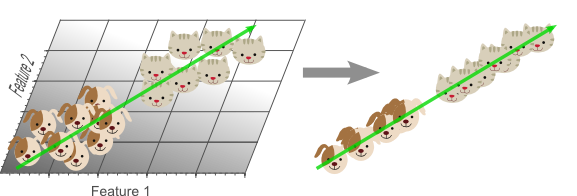
\includegraphics[scale=0.3]{img/2}  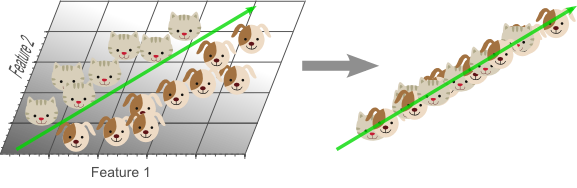
\includegraphics[scale=0.3]{img/1}
	 \end{center}
\end{frame}

\begin{frame}{SVD:  Faces dataset}
	 Main components: 
		 \begin{center}
			 	 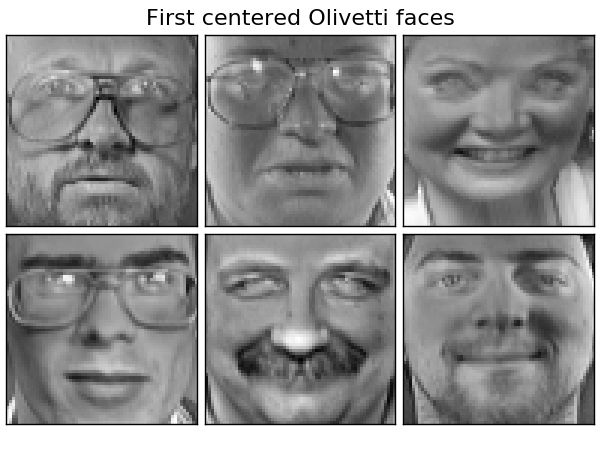
\includegraphics[scale=0.3]{img/face} ~~~ 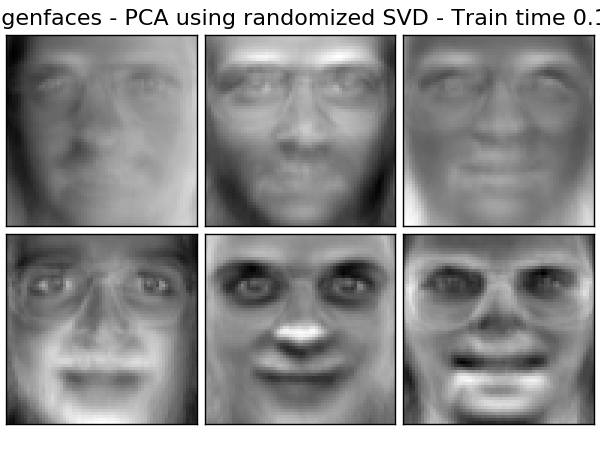
\includegraphics[scale=0.3]{img/svd_face}		 
		 \end{center}
	  Plot in 2d:
 		 \begin{center}
	  		 	 
\includegraphics[scale=0.25]{img/mnist} ~~~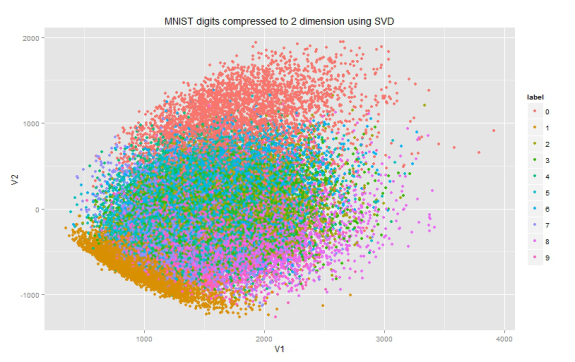
\includegraphics[scale=0.25]{img/svd_mnist}		 
 		 \end{center}
\end{frame}

\begin{frame}{Non-linear generalization}
	\begin{itemize}
		 \item What did we do wrong? Our picture mixes different classes and so on.
		 \item Let's try nonlinear generalization.
	\end{itemize}
	
	 \begin{center}
	 	 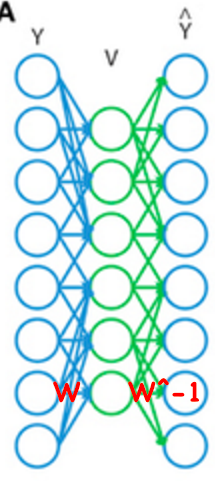
\includegraphics[scale=0.3]{img/fcautoenc1} ~~~ 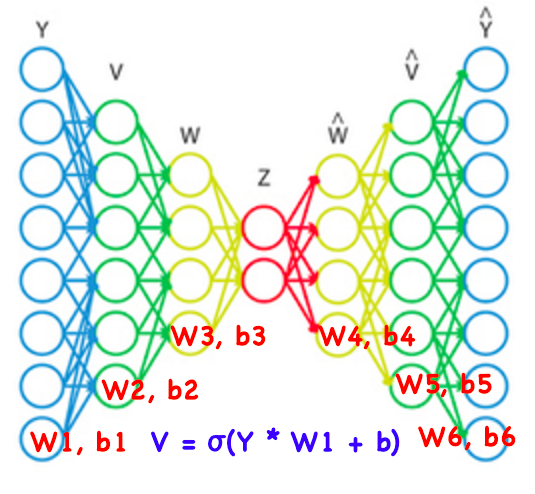
\includegraphics[scale=0.25]{img/fcautoenc2}		 
	 \end{center}
	
	\begin{itemize}
		 \item How to find $W_n, b_n$? 
		 \item Define loss function $L(Y, \hat{Y})$ and  use your favourite opt method.
	\end{itemize}
\end{frame}

\begin{frame}{Auto encoders example}
		 \begin{center}
		 	 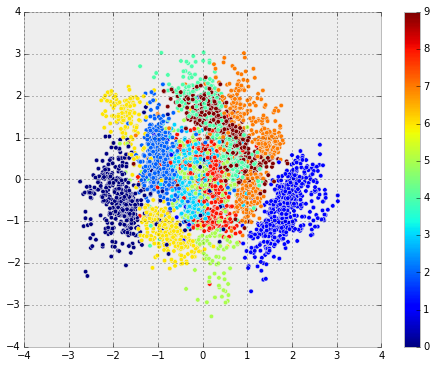
\includegraphics[scale=0.4]{img/autoenc}
		 \end{center}
	
	 \href{http://dpkingma.com/sgvb_mnist_demo/demo.html}{http://dpkingma.com/sgvb\_mnist\_demo/demo.html}
\end{frame}

\begin{frame}{Stochastic Neighbor Embedding}
	
	  X -- high dimensional obj and Y -- low dimensional ones, $\sigma$ -- width params
	
	$$ p_{j\mid i} = \frac{\exp(-\lVert\mathbf{x}_i - \mathbf{x}_j\rVert^2 / 2\sigma_i^2)}{\sum_{k \neq i} \exp(-\lVert\mathbf{x}_i - \mathbf{x}_k\rVert^2 / 2\sigma_i^2)}~~~ q_{j|i} = \frac{(-\lVert \mathbf{y}_i - \mathbf{y}_j\rVert^2)}{\sum_{k \neq i} (-\lVert \mathbf{y}_i - \mathbf{y}_k\rVert^2)}$$
	 
	\vspace{-0.1cm}
	$$KL(P||Q) = \sum_j\sum_{i} p_{i|j} \log \frac{p_{i|j}}{q_{i|j}} \rightarrow \min_q$$
	
	 \begin{center}
		 	 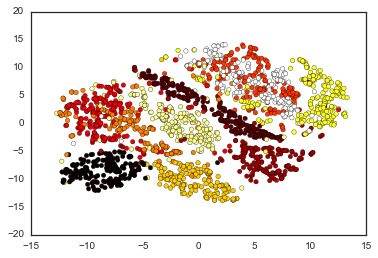
\includegraphics[scale=0.4]{img/tsne_mnist}
	 \end{center}
	
	Deep Neural Nets + t-SNE (modification of SNE with Student distr): \href{http://cs.stanford.edu/people/karpathy/cnnembed/}{http://cs.stanford.edu/people/karpathy/cnnembed/}
\end{frame}

\begin{frame}{CNN}
	 \begin{center}
	 	
	 	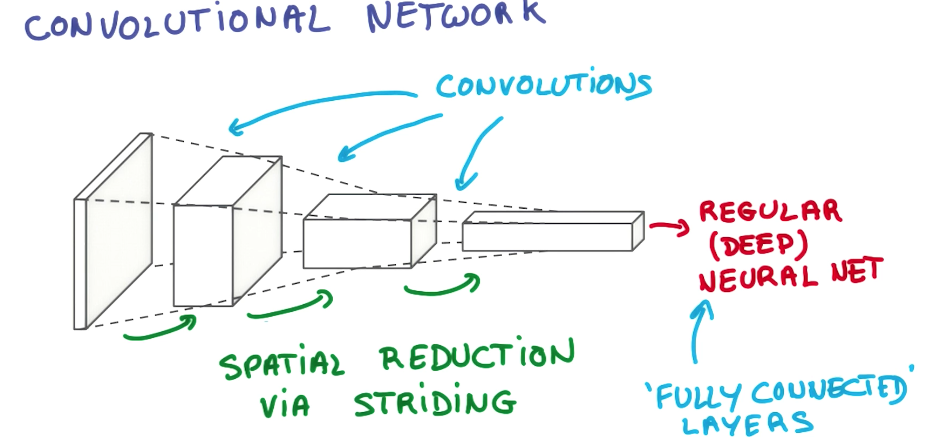
\includegraphics[scale=0.25]{img/cnn}
	 	
	 	
	 	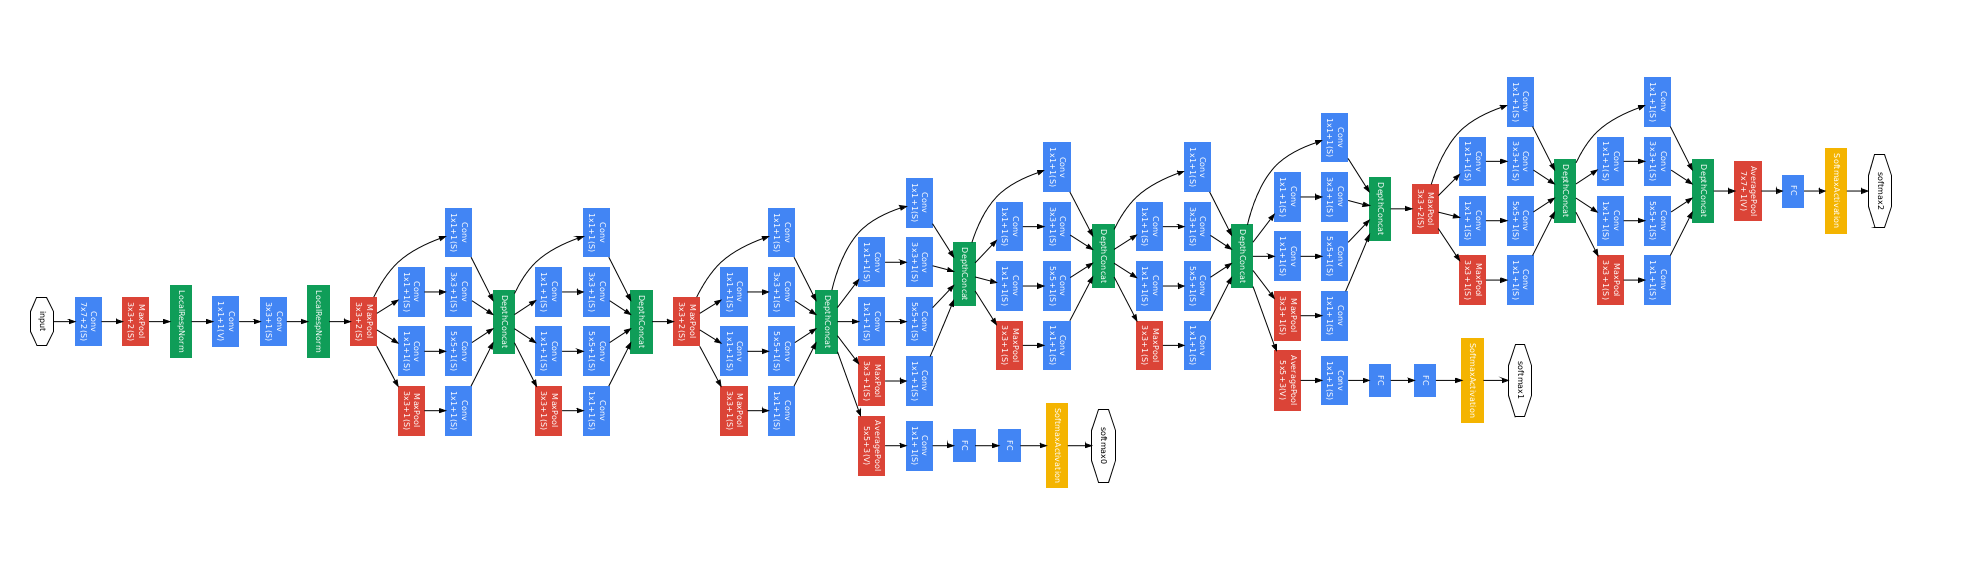
\includegraphics[scale=0.4]{img/gn}
	 \end{center}
\end{frame}

\begin{frame}{DNN Metric Learning Triplet Loss}
	
			 \begin{center}
			 	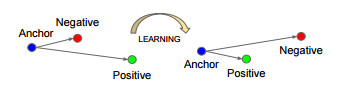
\includegraphics[scale=0.7]{img/ns}
			 \end{center}
	
		 \begin{center}
		 	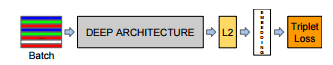
\includegraphics[scale=0.7]{img/tl2}
		 \end{center}
 The loss that is being minimized is then 
	 \begin{center}
	 	 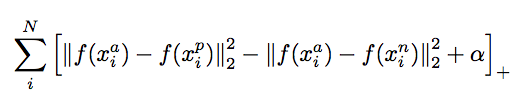
\includegraphics[scale=0.4]{img/tl}
	 \end{center}
\end{frame}

\begin{frame}{DNN Metric Learning Triplet Face and Music}
		 \begin{center}
		 	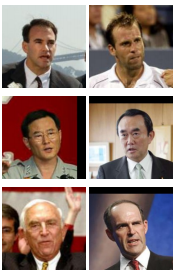
\includegraphics[scale=0.5]{img/face1} 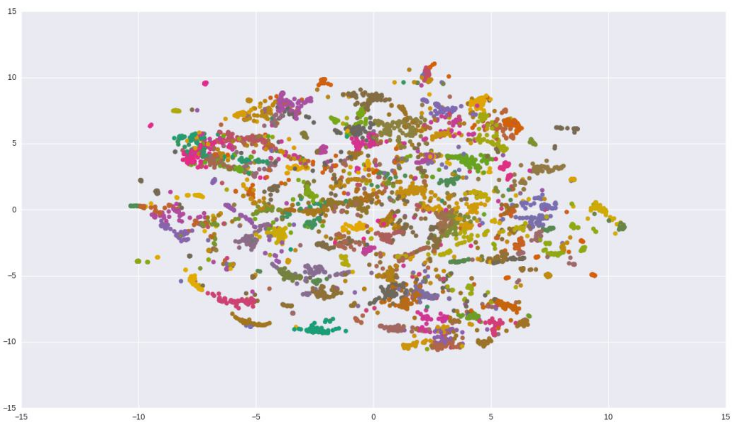
\includegraphics[scale=0.3]{img/music}
		 \end{center}
\end{frame}


\begin{frame}{High level}
	\begin{itemize}
		\item We have mapped each object into vector
		\item Let's train this vector for match complex object like words 		
	\end{itemize}
	
	\begin{center}
		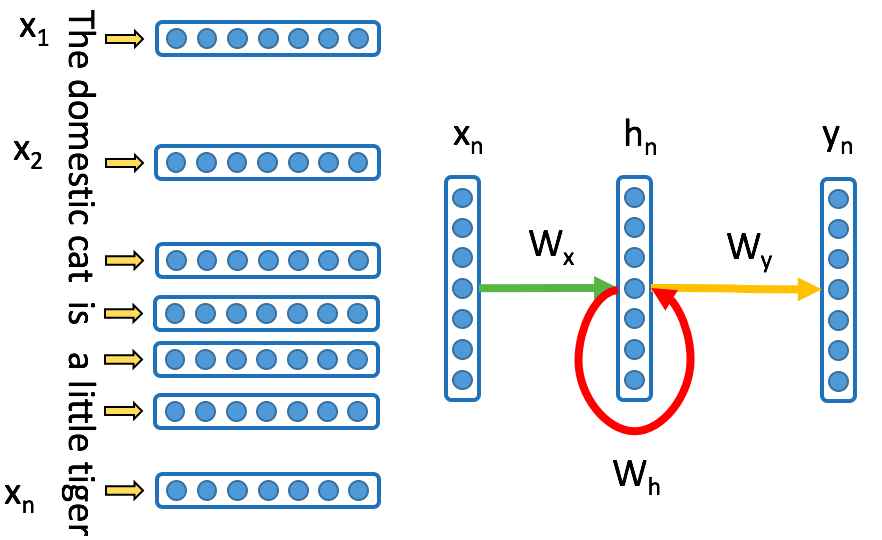
\includegraphics[scale=0.25]{img/recurrent_nn}
	\end{center}
	\vspace{-0.5cm}
	
	$$h_n = \textcolor{green}{W_x} x_n + \textcolor{red}{W_h}\sigma(h_{n-1})$$
	$$y_n = \sigma(\textcolor{notgreen}{W_y}  h_n)$$
\end{frame}


\begin{frame}{Word2Vec}
	\begin{itemize}
		\item Shallow Neural Net
				\begin{center}
					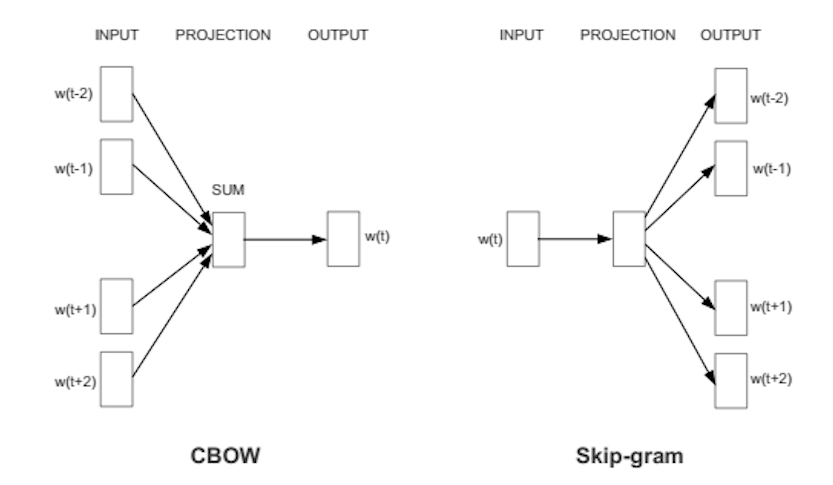
\includegraphics[scale=0.2]{img/w2vv}
				\end{center}
				
		\item Operations on embeddings are great
		\begin{center}
			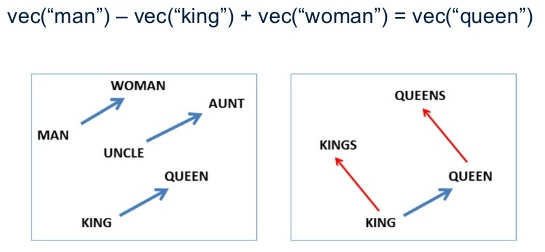
\includegraphics[scale=0.5]{img/w2v}
		\end{center}
		
	\end{itemize}
	\href{http://turbomaze.github.io/word2vecjson/}{http://turbomaze.github.io/word2vecjson/}
\end{frame}

\begin{frame}{Image2Text}
	\begin{itemize}
		\item Ok, we have a picture and want to represent in lower dim space
		\item Let's try to map picture to words sentence
	\end{itemize}
	\begin{center}
		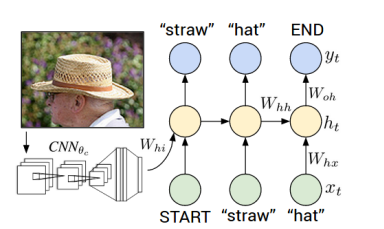
\includegraphics[scale=0.3]{img/nt}
		
		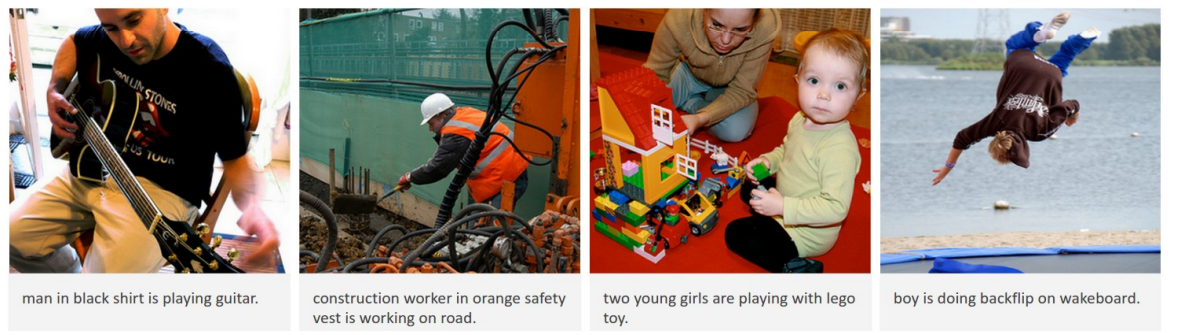
\includegraphics[scale=0.3]{img/ntw}
	\end{center}

	\href{http://cs.stanford.edu/people/karpathy/deepimagesent/}{http://cs.stanford.edu/people/karpathy/deepimagesent/}
	\href{http://cs.stanford.edu/people/karpathy/deepimagesent/rankingdemo/}{http://cs.stanford.edu/people/karpathy/deepimagesent/rankingdemo/}
\end{frame}

\begin{frame}{Generative Adversarial Networks}
	\begin{itemize}
		\item Image Generation is a lintel bit hardcore
		\item Most modern idea is like this
	\end{itemize}
	\begin{center}
		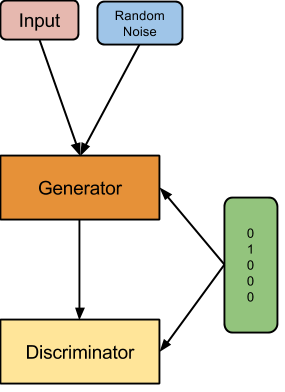
\includegraphics[scale=0.3]{img/gan2}
		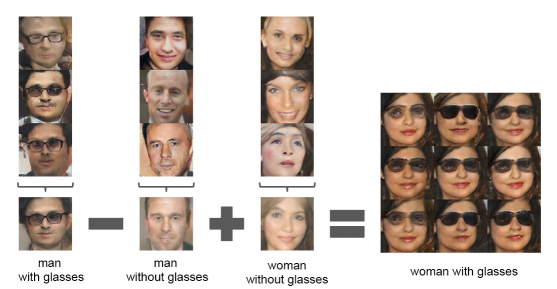
\includegraphics[scale=0.4]{img/gan1}
	\end{center}
\end{frame}

\begin{frame}{Text2Image}
		\begin{center}
			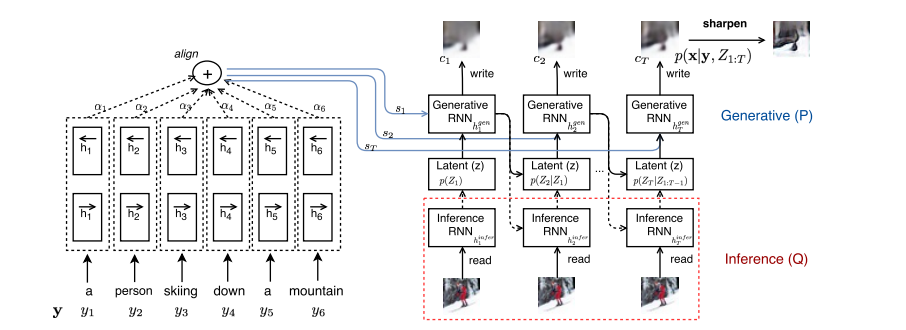
\includegraphics[scale=0.35]{img/t2i}
			
			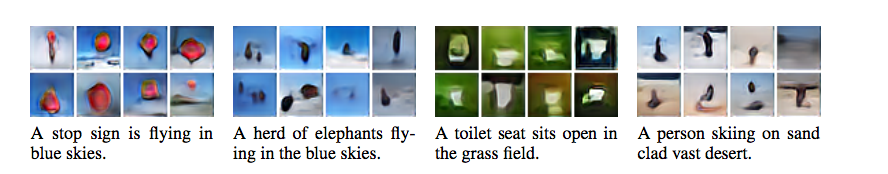
\includegraphics[scale=0.4]{img/t2ie.png}			
		\end{center}
	\href{https://arxiv.org/pdf/1511.02793v2.pdf}{https://arxiv.org/pdf/1511.02793v2.pdf}
\end{frame}

\begin{frame}{End} 
	\begin{center}				
		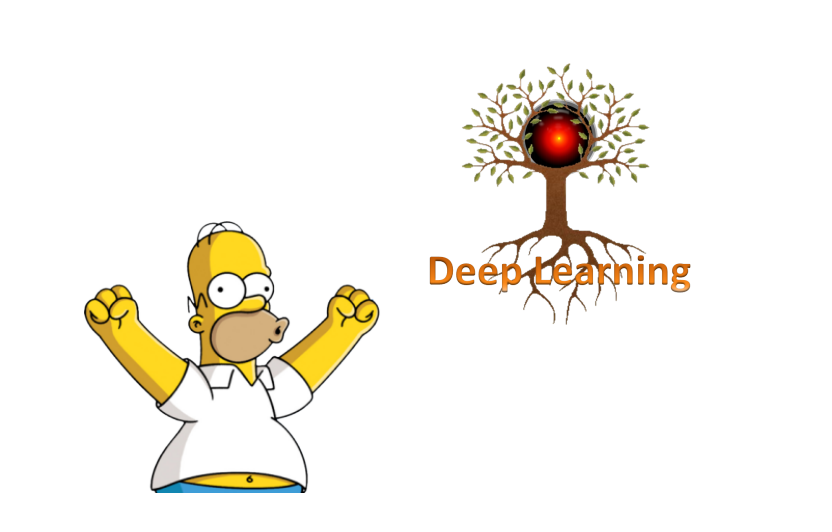
\includegraphics[scale=0.35]{img/csf}
		
		{\huge Current Status of your Field!}
		
		Thanks for your attention!
	\end{center}
\end{frame}


\end{document}

